\documentclass[sectionformat=exercise]{gadsescript}

\usetikzlibrary{shapes}

\setsemester{Winter Semester 2023/2024}%
\setuniversity{University of Konstanz}%
\setfaculty{Faculty of Science\\(Computer and Data Science)}%
\settitle{Elias Gestrich}
\setsubtitle{Turing Machines \& Decidability}

\begin{document}
\maketitle

\section{Turing Machine II}
\begin{enumerate}[label=\alph*)]
	\item ~
		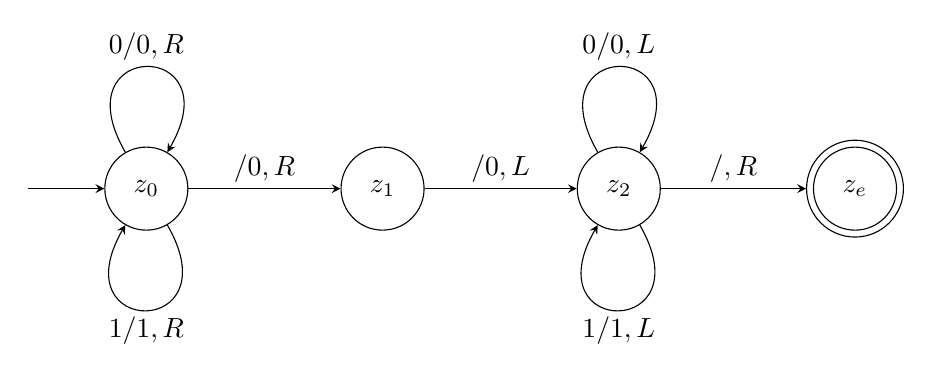
\begin{tikzpicture}
			\node[draw, circle, minimum size = 30] (z0) at (0,0) {$ z_0 $};
			\node[draw, circle, minimum size = 30] (z1) at (3,0) {$ z_1 $};
			\node[draw, circle, minimum size = 30] (z2) at (6,0) {$ z_2 $};
			\node[draw, circle, minimum size = 30] at (9,0) {$ z_e $};
			\node[draw, circle, minimum size = 35] (ze) at (9,0) {};
			\draw[-stealth] (-1.5, 0) -- (z0);
			\draw[-stealth] (z0) to[out=120,in=60,loop] node[midway, above, inner sep=2pt] {$ 0 / 0, R $} ();
			\draw[-stealth] (z0) to[out=-60,in=-120,loop] node[midway, below, inner sep=2pt] {$ 1 / 1, R $} ();
			\draw[-stealth] (z0) -- node[midway, above, inner sep = 2pt] {$ \square / 0, R $} (z1);
			\draw[-stealth] (z1) -- node[midway, above, inner sep = 2pt] {$ \square / 0, L $} (z2);
			\draw[-stealth] (z2) to[out=120, in=60, loop] node[midway, above, inner sep = 2pt] {$ 0 / 0, L $} (v1e);
			\draw[-stealth] (z2) to[out=-60, in=-120, loop] node[midway, below, inner sep = 2pt] {$ 1 / 1, L $} (v1e);
			\draw[-stealth] (z2) -- node[midway, above, inner sep = 2pt] {$ \square / \square, R $} (ze);
		\end{tikzpicture}
	\item $ z_0 10 \vdash 1 z_0 0 \vdash 10 z_0 \square \vdash 100z_1\square \vdash 10 z_2 00 \vdash 1 z_2 000 \vdash z_1 1000 \vdash z_1 \square 1000 \vdash z_e 1000 $
	\item $ z_0 110 \vdash 1 z_0 10 \vdash 11 z_0 0\vdash 110 z_0 \square \vdash 1100z_1\square \vdash 110 z_2 00 \vdash 11 z_2 000 \vdash 1 z_1 1000 \vdash z_1 11000 \vdash z_1 \square 11000 \vdash z_e 11000 $
	\item $ M_1 $ computes $ 4 \cdot the input $ as it adds two zeros to the end of a binary number.
\end{enumerate}


\section{Busy Beavers}
\begin{table}[H]
	\centering
	\begin{tabular}{cc|cc||c}
		$ z_1 $ & $ \square $ & $ z_2 $ & 1 & $ R $ \\
		$ z_1 $ & $ 1 $ & $ z_3 $ & 1 & $ L $ \\
		$ z_2 $ & $ \square $ & $ z_1 $ & 1 & $ L $ \\
		$ z_2 $ & $ 1 $ & $ z_2 $ & 1 & $ R $ \\
		$ z_3 $ & $ \square $ & $ z_1 $ & 1 & $ L $ \\
		$ z_3 $ & $ 1 $ & $ z_e $ & 1 & $ N $ \\
	\end{tabular}
	\caption{$ \delta $ }
	\label{tab:delta}
\end{table}

\section{Decidability}
\begin{enumerate}[label=\alph*)]
	\item \texttt{true}, since the definition of semi-decidability is that it stops if there is an answer but loops endlessly if there is no answer
	\item \texttt{unknown}, because the turing machine is semi-decidable, but there might be a turing machine that can identify if words are $ B $ or not and is decidable.
\end{enumerate}
\end{document}
